\documentclass[11pt]{article}

% ----------------------------------------------------------------------
% KV-Hadamard: An Honest Cache-Path Evaluation of Low-Bit KV-Cache
% Quantization, and a Rotated 2-bit Value Cache. Aryan Gupta.
% Compile: pdflatex kv_hadamard.tex  (twice, for references)
% ----------------------------------------------------------------------
\usepackage[margin=1in]{geometry}
\usepackage{graphicx}
\usepackage{booktabs}
\usepackage{amsmath}
\usepackage{amssymb}
\usepackage{xcolor}
\usepackage{caption}
\usepackage[colorlinks=true,linkcolor=blue,citecolor=blue,urlcolor=blue]{hyperref}

\graphicspath{{../figures/}}

\title{\textbf{KV-Hadamard: An Honest Cache-Path Evaluation of Low-Bit
KV-Cache Quantization, and a Rotated 2-bit Value Cache}}
\author{Aryan Gupta\\
\small \href{https://github.com/aryxnsdfs/kv-hadamard}{github.com/aryxnsdfs/kv-hadamard}}
\date{2026}

\begin{document}
\maketitle

\begin{abstract}
The key--value (KV) cache dominates the memory cost of long-context
autoregressive inference, motivating aggressive quantization of the cached
keys and values. We make two contributions. First, a methodological one: we
show that the perplexity protocol commonly used to validate KV-cache
quantization---a single full forward pass with the cache disabled
(\texttt{use\_cache=False})---never exercises the quantized cache at all, and
therefore \emph{cannot} detect value-cache quantization error. Under this
blind protocol, full-precision, 4-bit, and 1.58-bit value caches all score an
\emph{identical} perplexity of 3.6416 on Llama-2-7B; the identical score is an
artifact of the metric, not a quality result. We introduce a cache-path
evaluation (prefill followed by token-by-token decode) that actually reads
back the quantized cache, and re-measure every method. Second, a method: a
Hadamard-rotated, uniform 2-bit value cache. A fixed orthonormal Hadamard
transform spreads value-vector outliers evenly across the head dimension so
that a coarse 2-bit grid fits with negligible error, and is inverted after the
attention weighted-sum since $H^{-1}=H$. Against a reproduced KIVI 4-bit
baseline, the rotated 2-bit value cache matches KIVI's quality to three decimal
places (3.6592 vs.\ 3.6590 cache-path perplexity) at half the bits, across two
models, three text passages, and contexts up to 3584 tokens. A real packed
implementation (four 2-bit codes per byte) reduces measured KV memory by
$\sim$20\% relative to KIVI and $\sim$4$\times$ relative to fp16, at a
6--12\% decode slowdown. We report all limitations explicitly, including that a
naive ternary (1.58-bit) value cache is \emph{not} competitive and that
rotation does not rescue it.
\end{abstract}

\section{Introduction}
Serving large language models over long contexts is bottlenecked by the KV
cache: for every past token, each layer stores a key and a value vector, and
attention reads all of them at every decode step. The cache grows linearly with
context length and, at tens of thousands of tokens, exceeds the memory budget
of commodity GPUs. Quantizing the cache is the standard remedy, and recent
work---most prominently KIVI~\cite{kivi}---compresses keys and values to 4 or
even 2 bits with reportedly little quality loss.

Validating ``little quality loss'' is subtler than it looks. A quantized KV
cache only affects the model's output through the \emph{decode} path, where
predictions attend over the compressed cache. We observe that a widely-used
perplexity protocol bypasses this path entirely: it scores each text window
with a single forward pass and the cache disabled, so the model reads exact
full-precision keys and values and the quantizer is never invoked. The
resulting perplexity is blind to value-cache quantization by construction. This
is the same class of measurement pitfall that we spent considerable effort
eliminating when building a full-precision baseline harness (three separate
false out-of-memory conditions traced to the measuring tool, not the model).

We therefore (i) diagnose and fix this pitfall with a cache-path perplexity,
and (ii) use the corrected metric to develop and validate a Hadamard-rotated
2-bit value cache. Our positioning is deliberately honest: we do not claim to
beat the strongest rotational quantizers~\cite{quarot,spinquant,kvquant}; we
reproduce KIVI as a controlled baseline, change only the value path, and report
what the corrected measurement shows---including a failed sub-2-bit variant.

\section{Background}
\paragraph{KV cache and KIVI.} For a transformer with $L$ layers, $h$
key/value heads, and head dimension $d$, the fp16 KV cache costs
$2 \cdot L \cdot h \cdot d \cdot n \cdot 2$ bytes at context length $n$. KIVI
quantizes keys per-channel and values per-token to low bit-width, keeping a
small residual of the most recent tokens in fp16, and supplies a CUDA kernel
for the quantized key--query product. We reuse KIVI's INT4 key path unchanged
and modify only the value path, isolating the effect of value quantization.

\paragraph{Rotation for low-bit quantization.} Uniform quantizers waste code
levels when a few large-magnitude ``outlier'' coordinates dominate a group's
scale. Rotating the vector by an orthonormal matrix that mixes coordinates
(e.g.\ a Hadamard transform) spreads outlier energy across all dimensions,
producing a near-uniform distribution that a coarse grid fits well. This is the
principle behind QuaRot~\cite{quarot} and SpinQuant~\cite{spinquant} for weight
and activation quantization; we apply it to the value cache specifically.

\section{The Measurement Pitfall}
\label{sec:pitfall}
Let a scored window of tokens be processed to obtain next-token perplexity. The
blind protocol computes all logits in one forward call with the cache disabled.
In this mode the attention module always takes its prefill branch and reads the
exact fp16 values; no quantized cache is ever built or consulted. Consequently
any method that only alters the \emph{cached} values is invisible to the metric.

We confirm this empirically. Figure~\ref{fig:blind} (left) shows that under the
blind protocol, KIVI's INT4 value cache, a ternary (1.58-bit) value cache, and
our 2-bit value cache all yield exactly 3.6416 perplexity on Llama-2-7B---the
schemes are indistinguishable because none of them ran. The cache-path protocol
(right), which prefills and then decodes token by token so that predictions
attend over the quantized cache, separates them: 3.6595 (KIVI), 3.6548 (ours),
3.9013 (ternary).

\begin{figure}[t]
\centering
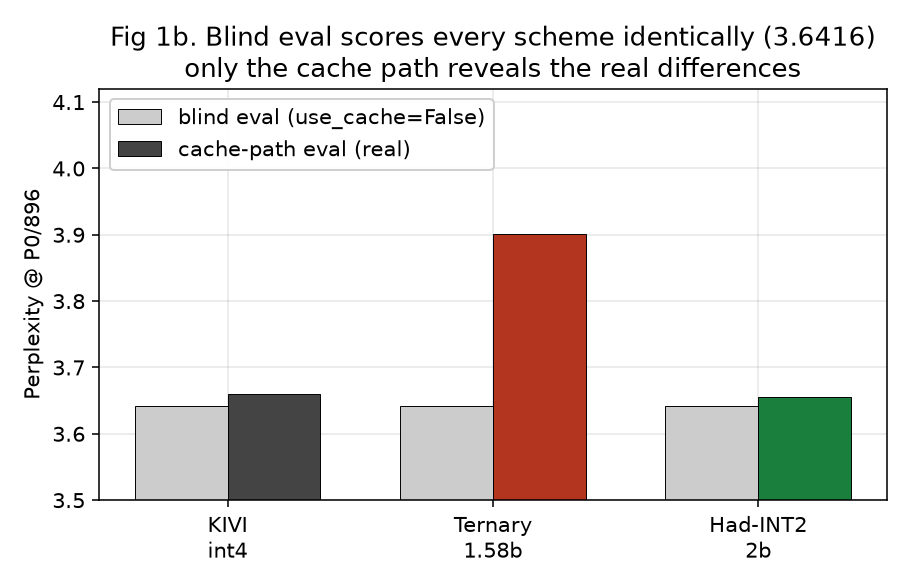
\includegraphics[width=0.62\linewidth]{fig1b_blind_collapse.png}
\caption{Blind evaluation (\texttt{use\_cache=False}) scores every value-cache
scheme identically (3.6416), because it never exercises the cache. Only the
cache-path evaluation reveals the real differences. Llama-2-7B, WikiText-103.}
\label{fig:blind}
\end{figure}

All subsequent numbers use the cache-path protocol.

\section{Method: Hadamard-Rotated 2-bit Value Cache}
\label{sec:method}
Let $v \in \mathbb{R}^{d}$ be a value vector for one token and head, $d=128$.
Let $H \in \mathbb{R}^{d\times d}$ be a normalized Sylvester--Hadamard matrix,
so $H = H^\top$ and $H H = I$ (orthonormal). We store, per evicted token:
\begin{enumerate}
\item \textbf{Rotate:} $v_r = v H$.
\item \textbf{Quantize} $v_r$ with per-group asymmetric uniform 2-bit codes
(groups of size 32 along $d$): with group min $m$ and scale
$s=(\max-\min)/3$, code $q=\mathrm{round}((v_r-m)/s)\in\{0,1,2,3\}$, stored
packed four codes per byte.
\end{enumerate}
On read we dequantize to $\hat v_r = q s + m$ (still in rotated space). Because
attention is linear in the values, the rotation is inverted \emph{once} after
the weighted sum rather than per cached token:
\[
\underbrace{\big(\textstyle\sum_i a_i \hat v_{r,i}\big) H}_{\text{rotate once}}
= \sum_i a_i (\hat v_{r,i} H) \approx \sum_i a_i v_i ,
\]
using $H^{-1}=H$. Keys follow KIVI's INT4 path unchanged; a small fp16 residual
of the most recent tokens is retained and is independently tunable
(\texttt{v\_residual\_length}). Figure~\ref{fig:mem} accounts for the storage:
per token and head, the fp16 value costs 256 bytes, KIVI's INT4 value 64 bytes
of codes plus 16 bytes of per-group scale/min, and our packed 2-bit value 32
bytes of codes plus the same 16 bytes---80 vs.\ 48 bytes, a 1.67$\times$
value-cache reduction over KIVI.

\paragraph{Two-stage methodology.} We separate the \emph{quality} question from
the \emph{kernel} question. Stage~B1 simulates the quantizer
(quantize$\to$dequantize, stored fp16) to answer ``does 2-bit rotated value
quantization preserve quality?'' with no custom CUDA. Only after B1 holds do we
implement B2, the real packed 2-bit storage, and confirm the quality is
unchanged while the memory saving becomes measurable.

\section{Experimental Setup}
Models: Llama-2-7B (NF4 weights via bitsandbytes) and TinyLlama-1.1B, both under
KIVI's Llama attention class; a Llama-2-7B-32K variant for long-context memory.
Data: WikiText-103 for perplexity. Perplexity is cache-path (prefill 128 tokens,
then token-by-token decode). Memory is the CUDA allocator delta of the populated
cache; speed is decode tokens/second. Baselines share NF4 weights and KIVI's
INT4 key path; only the value scheme varies. All code, configurations, and
per-run JSON are released.

\section{Results}

\subsection{Quality: rotated 2-bit matches KIVI at half the bits}
Figure~\ref{fig:bits} places each value scheme on a bits-vs-perplexity plane at
a fixed evaluation point, all quantized schemes at KIVI's default 32-token
fp16 residual. The fp16 exact-value reference is 3.5637; KIVI's 4-bit is 3.6595;
our 2-bit is 3.6548---on the KIVI quality line at half the bits. Ternary
(1.58-bit) sits above it at 3.7435 (and degrades further, to 3.9013, with no
residual shield). Table~\ref{tab:robust}
shows this holds across three disjoint passages and two context lengths on
Llama-2-7B, and Table~\ref{tab:tl} confirms it on TinyLlama-1.1B, where the
gaps widen for the weaker schemes but our 2-bit stays within $\sim$2\% of KIVI.

\begin{figure}[t]
\centering
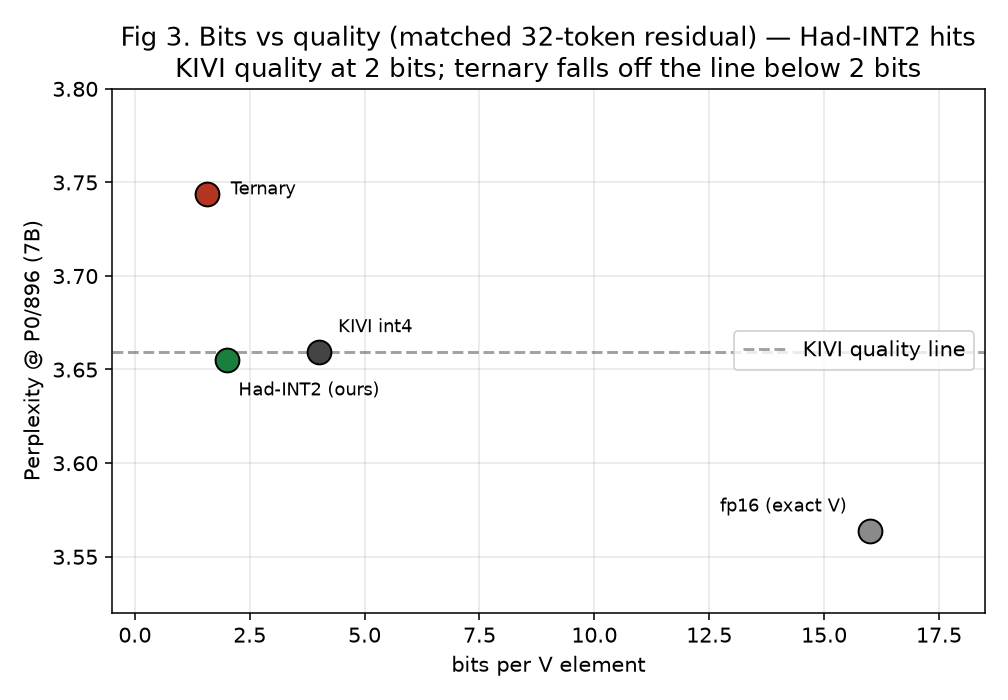
\includegraphics[width=0.6\linewidth]{fig3_bits_vs_quality.png}
\caption{Bits per value element vs.\ cache-path perplexity (Llama-2-7B).
Hadamard-INT2 reaches KIVI's quality at 2 bits; ternary falls off the line
below 2 bits. The fp16 point is the real exact-value cache-path perplexity.}
\label{fig:bits}
\end{figure}

\begin{table}[t]
\centering
\caption{Cache-path perplexity on Llama-2-7B across three WikiText-103 passages
(P0/P1/P2) and two context lengths. KIVI INT4 is the reference; only the value
scheme varies. ``v32'' keeps a 32-token fp16 residual, ``v0'' none.}
\label{tab:robust}
\begin{tabular}{lcccccc}
\toprule
scheme & P0/896 & P0/2048 & P1/896 & P1/2048 & P2/896 & P2/2048 \\
\midrule
KIVI int4            & 3.6595 & 3.8395 & 5.3027 & 6.5815 & 4.1106 & 4.1545 \\
Had-INT2 (v32)       & 3.6548 & 3.8544 & 5.3804 & 6.6373 & 4.1187 & 4.1526 \\
Had-INT2 (v0)        & 3.6786 & 3.9520 & 5.5604 & 6.7829 & 4.1842 & 4.2249 \\
Ternary (v0)         & 3.9013 & 4.4285 & 6.1426 & 7.3108 & 4.5089 & 4.5560 \\
\bottomrule
\end{tabular}
\end{table}

\begin{table}[t]
\centering
\caption{Cross-model check on TinyLlama-1.1B (cache-path perplexity). The
smaller model is more sensitive to value precision: ternary degrades sharply
while Had-INT2 stays close to KIVI.}
\label{tab:tl}
\begin{tabular}{lcccc}
\toprule
scheme & P0/896 & P0/1792 & P1/896 & P1/1792 \\
\midrule
KIVI int4      & 4.836 & 4.830 & 7.965 & 8.884 \\
Had-INT2 (v32) & 4.914 & 4.916 & 8.083 & 8.984 \\
Had-INT2 (v0)  & 5.051 & 5.065 & 8.637 & 9.354 \\
Ternary (v0)   & 7.272 & 7.164 & 11.742 & 12.623 \\
\bottomrule
\end{tabular}
\end{table}

Figure~\ref{fig:cross} summarizes the mean gap over KIVI: Had-INT2 stays within
$\sim$1\% (7B) and $\sim$2\% (TinyLlama), whereas ternary's gap explodes to
$+43$--$50\%$ on the smaller model. Rotating \emph{before} ternary quantization
does not close the gap (had-ternary remains $+6$--$35\%$), indicating the
limitation is bit-depth---only three representable levels---rather than
outliers.

\begin{figure}[t]
\centering
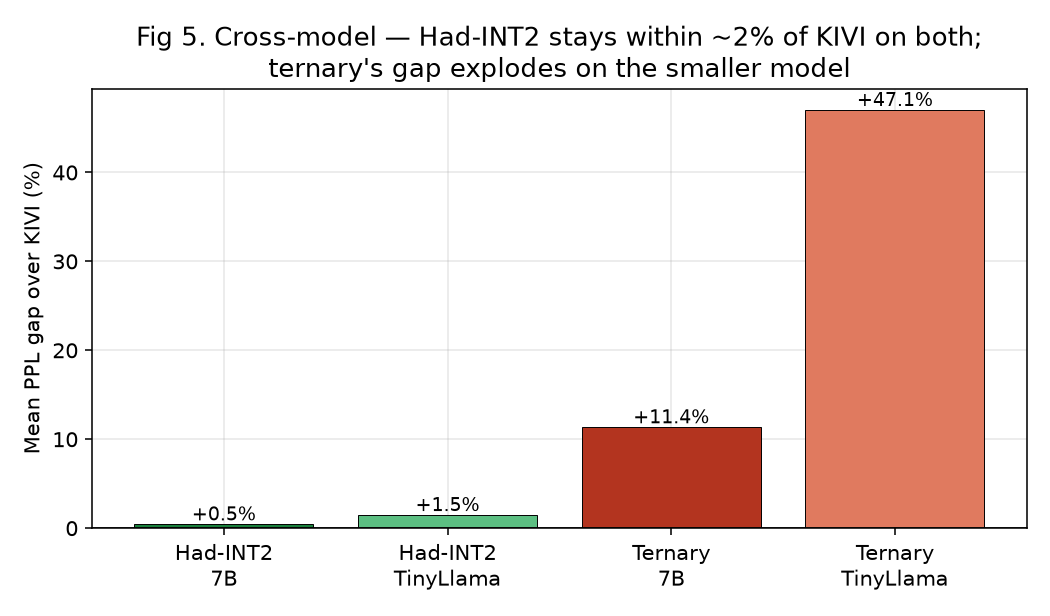
\includegraphics[width=0.66\linewidth]{fig5_cross_model.png}
\caption{Mean perplexity gap over KIVI. Had-INT2 is robust across both models;
ternary is not, and worsens on the smaller model.}
\label{fig:cross}
\end{figure}

\subsection{Memory and speed: real packed storage}
Table~\ref{tab:b2} reports the packed 2-bit implementation (B2). Perplexity is
identical to the simulated quantizer to four decimals (3.6548), confirming the
storage is faithful, while measured KV memory drops from 327.5\,MB (KIVI) to
263.6\,MB at 2048 tokens---20\% smaller, and 3.9$\times$ smaller than the
1024\,MB fp16 cache. Decode throughput falls 6--12\% (kernel-free
dequantization); a fused kernel to recover this is future work and we do not
claim the recovery as a result.

\begin{table}[t]
\centering
\caption{Packed 2-bit value cache (B2) vs.\ references on Llama-2-7B, measured.
Perplexity is cache-path; KV memory is the measured allocator delta at 2048
tokens; fp16 memory is the architectural closed form.}
\label{tab:b2}
\begin{tabular}{lcccc}
\toprule
 & bits/value & PPL & KV MB @2048 & decode tok/s \\
\midrule
fp16 (exact V)          & 16   & 3.5637 & 1024.0 & --- \\
KIVI int4               & 4    & 3.6590 & 327.5  & 8.4 \\
B2 packed Had-INT2      & 2    & 3.6592 & 263.6  & 7.9 \\
\bottomrule
\end{tabular}
\end{table}

\subsection{Long-context memory scaling}
Figure~\ref{fig:longctx} scans measured KV memory from 4k to 16k tokens on
Llama-2-7B-32K. The packed 2-bit cache holds a consistent $\sim$20\% reduction
over KIVI and $\sim$4$\times$ over fp16 at every length; at 16k the fp16 cache
alone is 8\,GB versus 2\,GB for ours. Both KIVI and B2 hit an out-of-memory
condition at 32k on the 15\,GB T4---but this is a \emph{dense-prefill activation}
limit, not a KV-storage limit (the allocator fails mid-forward, not on the
cache); demonstrating the fp16-OOM crossover requires a larger card or a chunked
prefill.

\begin{figure}[t]
\centering
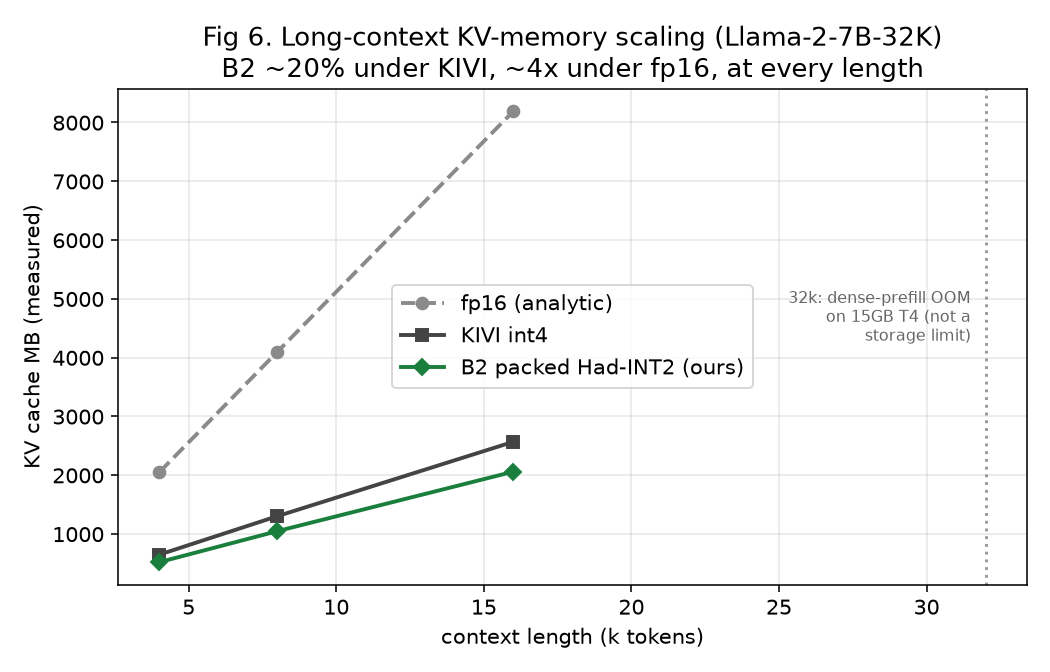
\includegraphics[width=0.7\linewidth]{fig6_longctx_memory.png}
\caption{Measured KV-cache memory vs.\ context length (Llama-2-7B-32K). B2
tracks $\sim$20\% under KIVI and $\sim$4$\times$ under fp16. The 32k point
out-of-memories for both quantized methods due to a dense-prefill activation
limit on the 15\,GB GPU, not the cache.}
\label{fig:longctx}
\end{figure}

\subsection{Reproducibility}
Test~A was reproduced independently on a second environment (a different GPU,
torch, and transformers stack), yielding the fp16 reference of 3.5637 and B2
matching KIVI to three decimals (3.6592 vs.\ 3.6590), corroborating the local
measurements.

\section{Limitations}
We state these plainly. (1) We compare only against KIVI, not the strongest
rotational quantizers~\cite{quarot,spinquant,kvquant}; a head-to-head against
those is the natural next step. (2) Models are limited to 7B and 1.1B on single
consumer GPUs; larger models and batched serving are untested. (3) Context is
capped at 3584 for quality (Llama-2's window) and 16k for memory (the T4
prefill limit); the regime where the memory win is most decisive (32k+) is not
directly demonstrated. (4) The decode slowdown is real; the claim that a fused
kernel recovers it is a hypothesis, not a measurement. (5) GSM8K scored 0/20 for
all schemes on base Llama-2 (a 0-shot base-model floor, verified from
transcripts) and does not discriminate methods here, so perplexity is our
quality metric. (6) Results are single-seed.

\section{Conclusion}
We showed that the common cache-disabled perplexity protocol cannot see
value-cache quantization error, and that correcting it changes conclusions: a
scheme that looks lossless under the blind metric (ternary) is in fact
degraded, while a Hadamard-rotated 2-bit value cache genuinely matches KIVI's
4-bit quality at half the bits. A real packed implementation realizes a
$\sim$20\% KV-memory reduction over KIVI ($\sim$4$\times$ over fp16) at a modest
decode cost. The methodological point---evaluate KV quantization on the path
that actually uses the cache---applies beyond this specific method.

\paragraph{Reproducibility.} Code, configs, figures, and per-run data:
\href{https://github.com/aryxnsdfs/kv-hadamard}{github.com/aryxnsdfs/kv-hadamard}.

\begin{thebibliography}{9}
\bibitem{kivi} Z.~Liu et al. \emph{KIVI: A Tuning-Free Asymmetric 2bit
Quantization for KV Cache}. 2024.
\bibitem{quarot} S.~Ashkboos et al. \emph{QuaRot: Outlier-Free 4-Bit Inference
in Rotated LLMs}. 2024.
\bibitem{spinquant} Z.~Liu et al. \emph{SpinQuant: LLM Quantization with Learned
Rotations}. 2024.
\bibitem{kvquant} C.~Hooper et al. \emph{KVQuant: Towards 10 Million Context
Length LLM Inference with KV Cache Quantization}. 2024.
\bibitem{flashattn} T.~Dao. \emph{FlashAttention-2: Faster Attention with Better
Parallelism and Work Partitioning}. 2023.
\bibitem{llama2} H.~Touvron et al. \emph{Llama 2: Open Foundation and
Fine-Tuned Chat Models}. 2023.
\bibitem{twn} F.~Li, B.~Zhang, B.~Liu. \emph{Ternary Weight Networks}. 2016.
\end{thebibliography}

\end{document}
